\chapter{The CERN Large Hadron Collider}
\label{sec:02_lhc}

The Large Hadron Collider (LHC) is a proton-proton collider located at CERN on the border of Switzerland and France (Figure~\ref{fig:02_lhc_geneva}).
It is the largest and highest energy particle accelerator in the world, with a circumference of 27.6\unit{km} and a center-of-mass (COM) energy of 13.6\unit{TeV}, reproducing energies in the universe $10^{-11}$ seconds after the Big Bang.

\begin{figure}[ht]
    \centering
    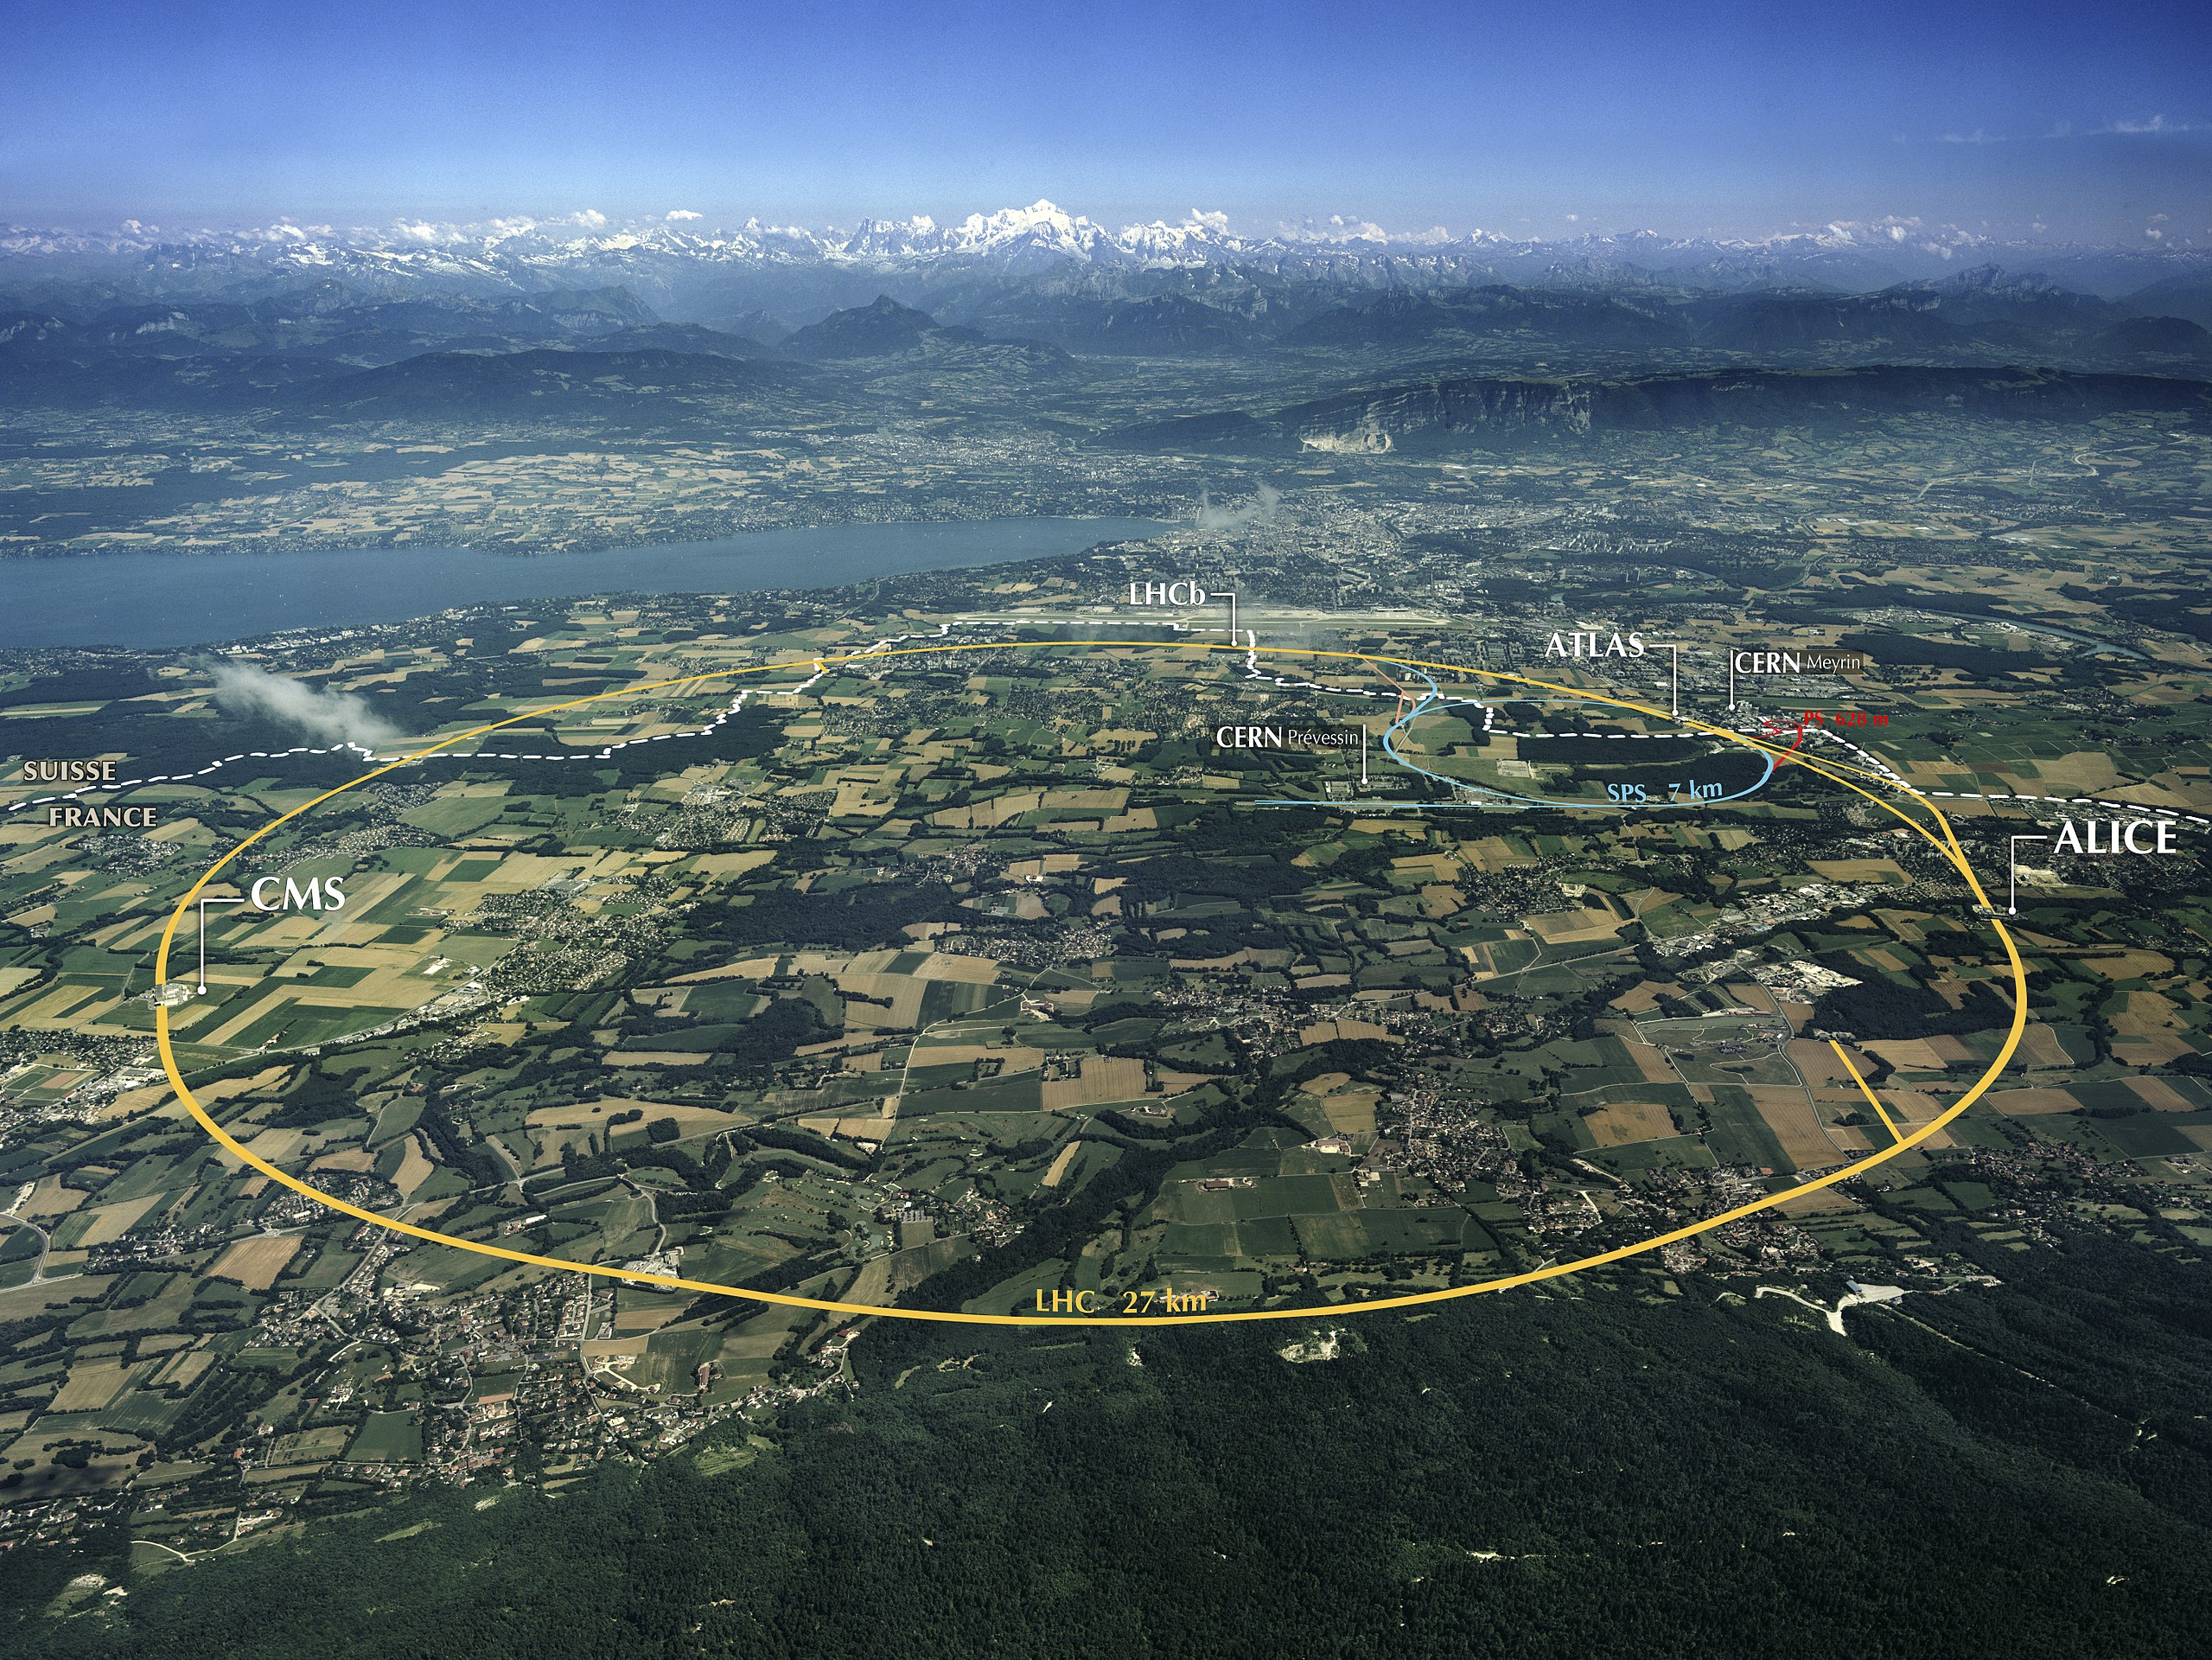
\includegraphics[width=\textwidth]{figures/02-CMS/lhc/lhc_geneva.jpg}
    \caption{Outline of the LHC overlaid on a satellite image of Switzerland and France.}
    \label{fig:02_lhc_geneva}
\end{figure}

The tunnel was initially built for the large electron-positron collider (LEP), which operated from 1989 to 2000.
Being point particles and not interacting with the strong force, electrons and positrons produce ``clean'' collisions (i.e., with low background) and can be simulated with relative ease; thus, LEP allowed high precision measurements of the electroweak sector of the standard model (SM), as discussed in Chapter~\ref{sec:01_sm}.
The drawback, however, is that due to the power loss from synchotron radiation, which scales as $\propto ($mass of the accelerated particle$)^{-4}$, their low mass limits the COM energy that can be attained with electron-positron colliders.

Protons, on the other hand, are composite particles and produce ``noisy'', high-multiplicity collisions, but are $2000\times$ more massive and, hence, can be accelerated to much higher energies.
% The $1000\times$ higher mass of protons allows for much higher energies.
This is why, from early on, the LEP tunnel had also been proposed as a site for a future \textit{hadron-hadron} collider, which could achieve an order-of-magnitude greater energy than the previous energy-frontier machine, the Fermilab Tevatron.
The LHC was eventually approved in 1994 and was built in collaboration with over 100 countries at CERN between 1998 and 2008.
It is primarily a proton-proton collider, designed with the goal of accelerating each proton to $7\TeV$, for a COM energy of $14\TeV$, to explore the \TeV energy scale for the first time.
It also, less frequently, collides heavy ions to study QCD and the quark-gluon plasma inside nuclei.

The collisions occur at four interaction points around the ring and are observed by a total of nine detectors: two large general-purpose detectors, CMS and ATLAS, two more specialized detectors, ALICE and LHCb, for heavy-ion- and b-physics, respectively, and five smaller scale experiments, TOTEM, LHCf, MoEDAL, FASER, and SHiP.
In this section, we describe the LHC accelerator in Section~\ref{sec:02_lhc_accelerator} and the overall number of collisions, quantified as ``integrated luminosity'', it has delivered and expects to deliver in Section~\ref{sec:02_lhc_luminosity}.

\section{The accelerator}
\label{sec:02_lhc_accelerator}

The overall LHC accelerator complex is shown in Figure~\ref{fig:02_lhc_accelerator}.
Protons are first extracted from a hydrogen gas bottle through a duoplasmatron ion source~\cite{wolf1995handbook} as a low energy beam of around 100\unit{keV}.
They are then accelerated through a series of ``injectors'' (Figure~\ref{fig:02_lhc_injectors}): first through a linear accelerator (LINAC) up to 50\MeV; then a proton synchotron booster (PSB) up to 1.4\GeV; the proton synchotron (PS) up to 26\GeV; and finally through the super proton synchotron (SPS) up to 450\GeV, after which the protons are transferred to the LHC ring.

\begin{figure}[ht]
    \centering
    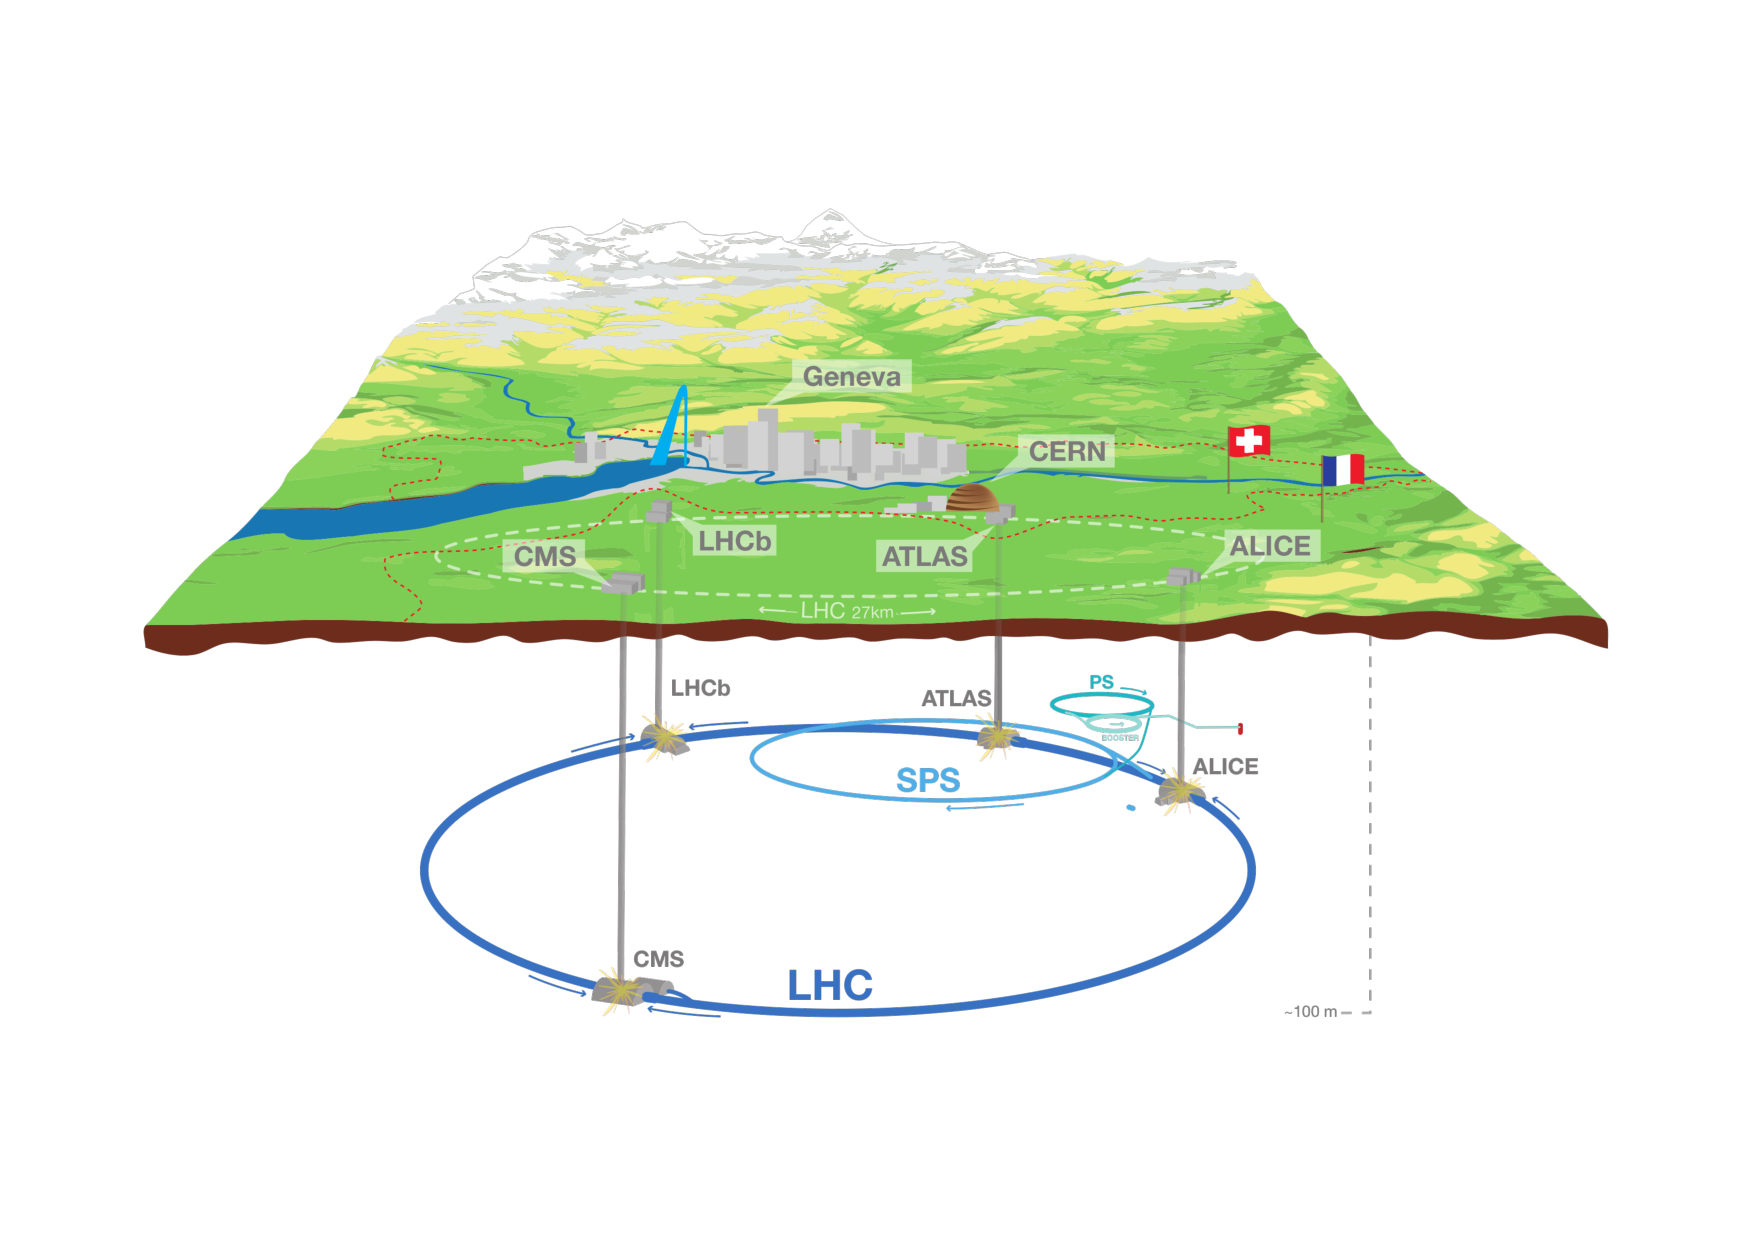
\includegraphics[trim=0pt 80pt 0pt 150pt, width=\textwidth]{figures/02-CMS/lhc/LHC_overall.pdf}
    \caption{Diagram of the LHC accelerator complex adapted from Ref.~\cite{Mouche:1708847}, depicting the initial proton source (in red), LINAC, proton synchotron booster, PS, SPS, LHC, and the four main experiments: CMS, ATLAS, ALICE, and LHCb.}
    \label{fig:02_lhc_accelerator}
\end{figure}

\begin{figure}[ht]
    \centering
    \captionsetup{justification=centering}
    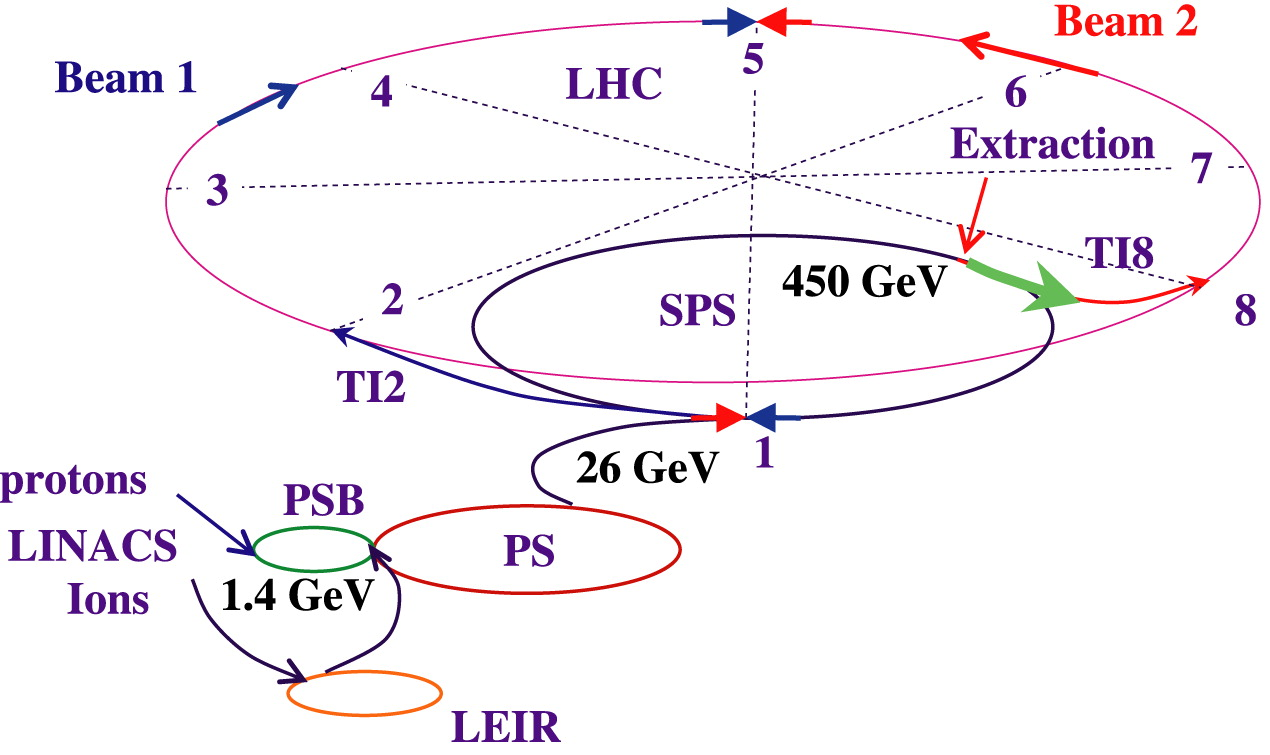
\includegraphics[width=\textwidth]{figures/02-CMS/lhc/lhc_injectors.jpg}
    \caption{Schematic of the LHC injectors, reproduced from Ref.~\cite{Bruning:2012zz}.}
    \label{fig:02_lhc_injectors}
\end{figure}

Unlike particle-antiparticle colliders, like the Tevatron, which can accelerate both beams in the same ring with the same magnet system, the proton-proton collisions at the LHC require opposite magnetic fields for the beams before their collision.
The benefit, of course, is the ease of producing protons compared to antiprotons, allowing for far higher luminosities.
Due to the small 3.7\unit{m} internal diameter of the existing LEP tunnel, it was not possible to install two separate rings for the two counter-rotating beams; instead, a twin-bore magnet design~\cite{Blewett:1971zzb} was chosen to accommodate both in the same ring (Figure~\ref{fig:02_lhc_twinbore}) with two separate vacuum chambers and superconducting coils.

A total of 1,232 such superconducting NbTi dipole magnets are installed around the ring to maintain the circular trajectory of the protons, as well as 392 quadrupole and higher multipole-order magnets to focus the beams.
The maximum beam momentum $p$ is limited by the bending radius ($\rho$) and the bending field strength ($B$) of the dipole magnets, as~\cite{Bruning:2012zz}:
\begin{equation}
    p [\GeV / c] = B [\unit{T}] \rho [\unit{m}] / 3.336.
\end{equation}
For the LHC tunnel, $\rho$ is $2.8\unit{km}$; hence, to achieve 7\TeV protons, the dipole magnets were designed to achieve a field strength of 8.33\unit{T} (requiring liquid helium cooling to a temperature of 1.9\unit{K} to maintain superconductivity).
However, due to imperfections in some magnets, the LHC initially operated at 3.5--4\TeV per beam in Run 1 (2010--2012), then 6.5\TeV in Run 2 (2015--2018), and currently 6.8\TeV in Run 3 (2022--2026).

\begin{figure}[ht]
    \centering
    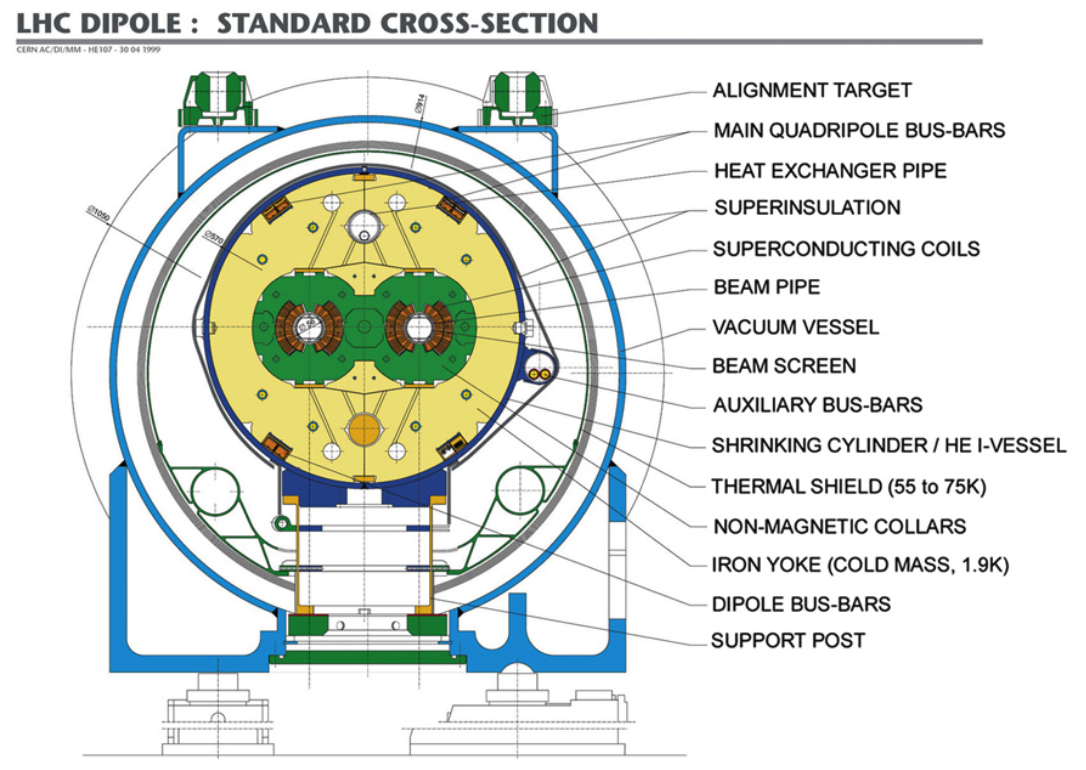
\includegraphics[width=0.49\textwidth]{figures/02-CMS/lhc/dipole_crossection.png}
    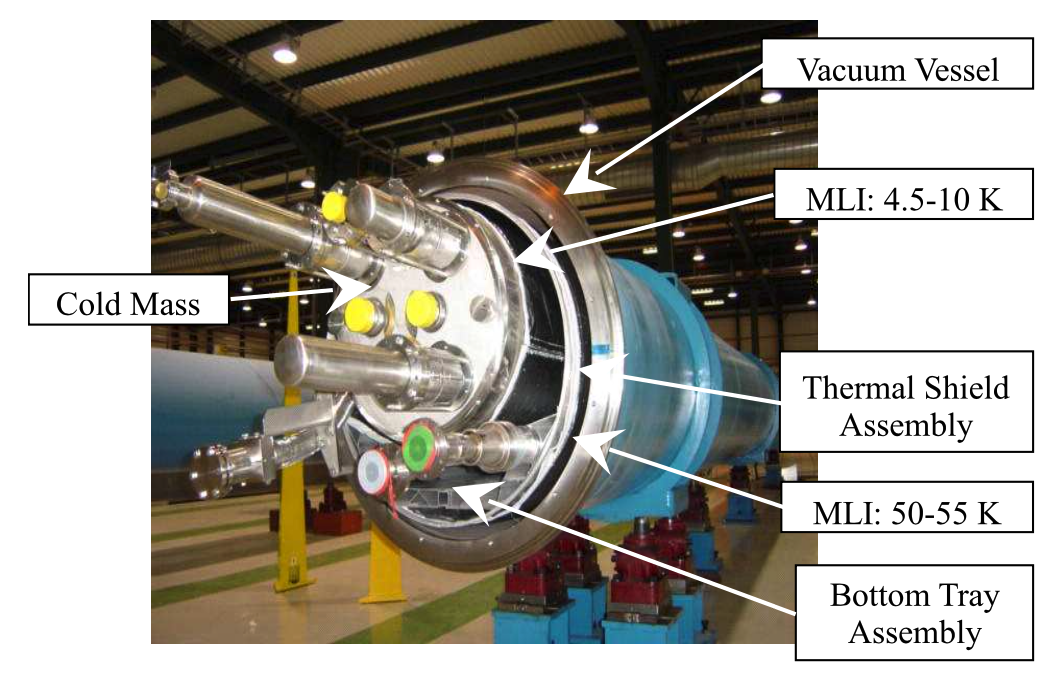
\includegraphics[width=0.49\textwidth]{figures/02-CMS/lhc/magnet.png}
    \caption{Diagram of the cross-section of the twin-bore LHC dipole magnets (left) and an image of an actual LHC dipole magnet (right), reproduced from Ref.~\cite{Evans:2008zzb}.}
    \label{fig:02_lhc_twinbore}
\end{figure}

The LHC layout comprises eight arcs and eight $\sim 500\unit{m}$ long straight sections.
The two beams are diverted and collided in four of the straight sections, called ``interaction points'' (IPs), where the detectors are located (Figure~\ref{fig:02_lhc_octants}).
The other four straight sections are used for utilities, such as the beam dump and collimation systems.

\begin{figure}[ht!]
    \centering
    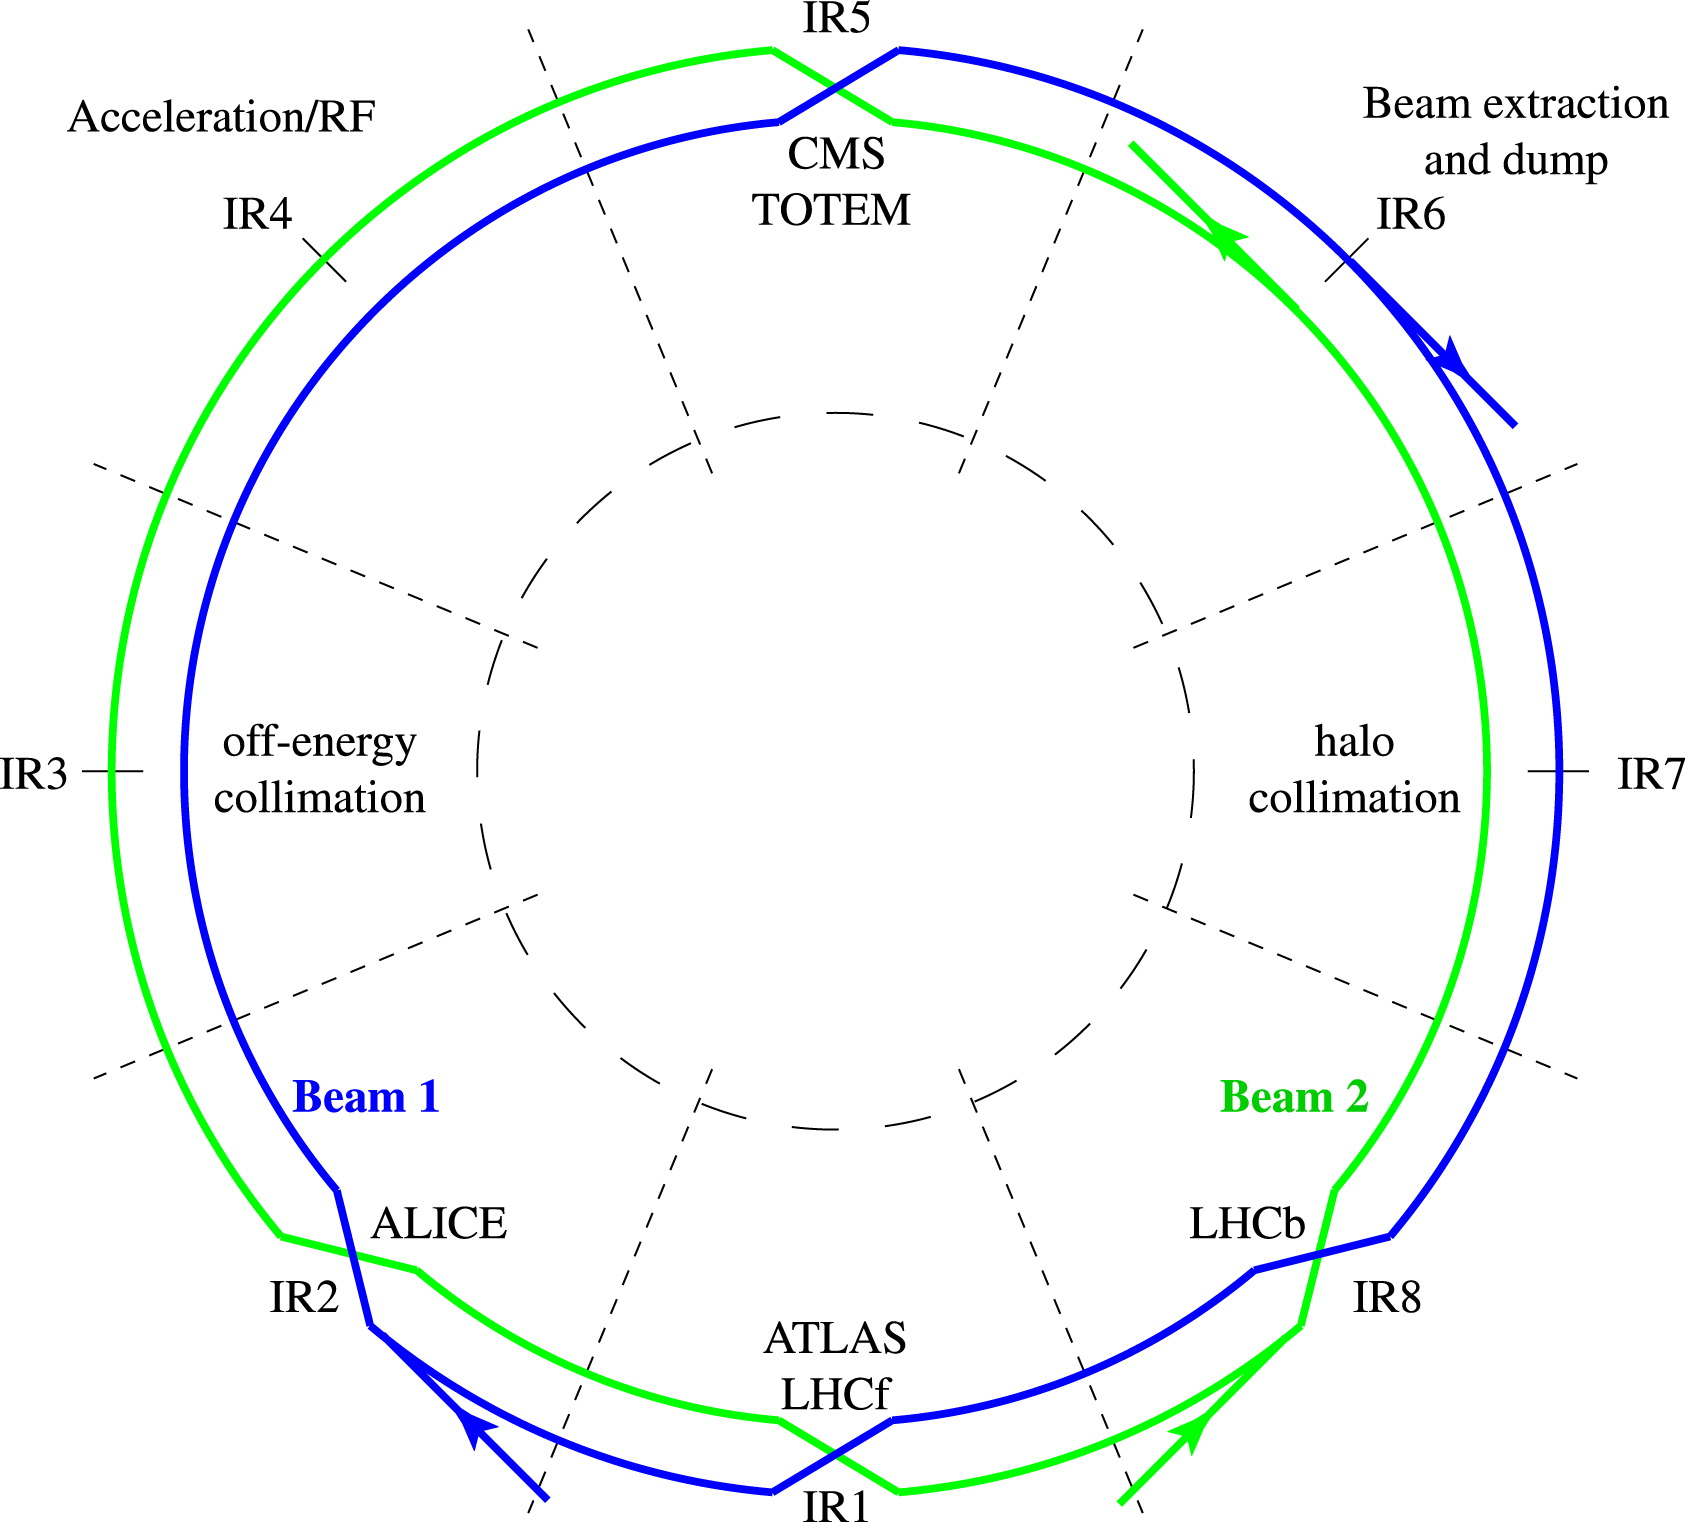
\includegraphics[width=\textwidth]{figures/02-CMS/lhc/lhc_octants.jpg}
    \caption{Schematic of the LHC layout showing the two proton beams in green and blue and its division into eight octants, reproduced from Ref.~\cite{Bruning:2012zz}.}
    \label{fig:02_lhc_octants}
\end{figure}

The protons are accelerated and collided in ``bunches'' of $10^{11}$ protons each, with a separation of 25\unit{ns} between bunches.
The greater the number of protons per bunch and frequency of bunches, the greater the total luminosity of the collider.
Each bunch is accelerated and phase-focused longitudinally by a series of 16 superconducting radiofrequency (RF) cavities into separate ``RF buckets''.
The RF-frequency of the cavities is 400\unit{MHz}, corresponding to a theoretical minimum spacing in time of 2.5\unit{ns} between RF buckets / bunches.
The LHC opts for the 10-bucket spacing of 25\unit{ns} to avoid ``parasitic'' collisions between bunches~\cite{Bruning:2012zz}.
With this spacing, the maximum number of bunches in the ring is 2808.


\section{Luminosity and timeline}
\label{sec:02_lhc_luminosity}

As discussed in Chapter~\ref{sec:01_qft}, the number of scattering events we expect is the product of the scattering cross section and the \textit{luminosity} ($L$) of the particle beams (Eq.~\ref{eq:01_qft_interactions_cross_section_luminosity}).
Cross sections are typically given in units of barn (b), where $1\unit{b} = 10^{-28}\unit{m}^2$, and thus the luminosity often in inverse barns (b$^{-1}$).
For a circular collider, the instantaneous luminosity is given by~\cite{Bruning:2012zz}:
\begin{equation}
    \label{eq:02_lhc_luminosity}
    L = \frac{N_1 N_2 n_b f_{\mathrm{rev}}}{A},
\end{equation}
where $N_1$ and $N_2$ are the number of protons in each bunch, $n_b$ is the number of bunches, $f_{\mathrm{rev}}$ is the revolution frequency of the beams, and $A$ is the effective beam overlap area at the interaction point.
This is why the LHC design aims to maximize the number of protons per bunch, the number of bunches, and the frequency of bunches, while focusing and aligning the beams as much as possible at the interaction point.
The instantaneous luminosity of pp collisions at the LHC has increased steadily from a peak of $2.1\times10^{32}$\unit{cm$^{-2}$s$^{-1}$} in 2010 to around $2.5\times10^{34}$\unit{cm$^{-2}$s$^{-1}$} in 2022--24~\cite{cmslumi2024}.
Higher luminosity also leads to a higher rate of simultaneous pp collisions during a single bunch crossing, called \textit{pileup}, which results in background noise to the detectors.
As shown in Figure~\ref{fig:02_lhc_pileup}, the average rate of pileup in CMS has ranged from $10$ in 2011 to around $57$ in 2024.

The total luminosity delivered by the LHC is the integral of the above over time, called the \textit{integrated luminosity}, and is shown in Figure~\ref{fig:02_lhc_luminosity} along with the projection up to 2041.\footnote{Note that this projection has not been updated to reflect the decision made in September 2024 to extend Run 3 up to 2026 and delay the start of Run 4 to 2030.}
So far, the LHC has delivered around 60\unit{fb$^{-1}$} of integrated luminosity at $7$ or $8\TeV$ COM to the CMS and ATLAS experiments in Run 1, 138\unit{fb$^{-1}$} at $13\TeV$ in Run 2, and is currently aiming for around 300\unit{fb$^{-1}$} at $13.6\TeV$ in Run 3.
After this, (tentatively) between 2026 and 2030, the LHC will undergo a significant upgrade aiming to deliver an order of magnitude more luminosity in Runs 4--6, between $5$--$7\times10^{34}$\unit{cm$^{-2}$s$^{-1}$} instantaneously, integrated to around 3000\unit{fb$^{-1}$}!
This is called the High-Luminosity LHC (HL-LHC) upgrade~\cite{HL-LHC} (see Figure~\ref{fig:02_lhc_plan}), and is expected to allow access to rare processes such as Higgs boson pair production; however, it also entails major accelerator, detector, and computational challenges to effectively deliver and exploit the increased luminosity.

\begin{figure}[ht!]
    \centering
    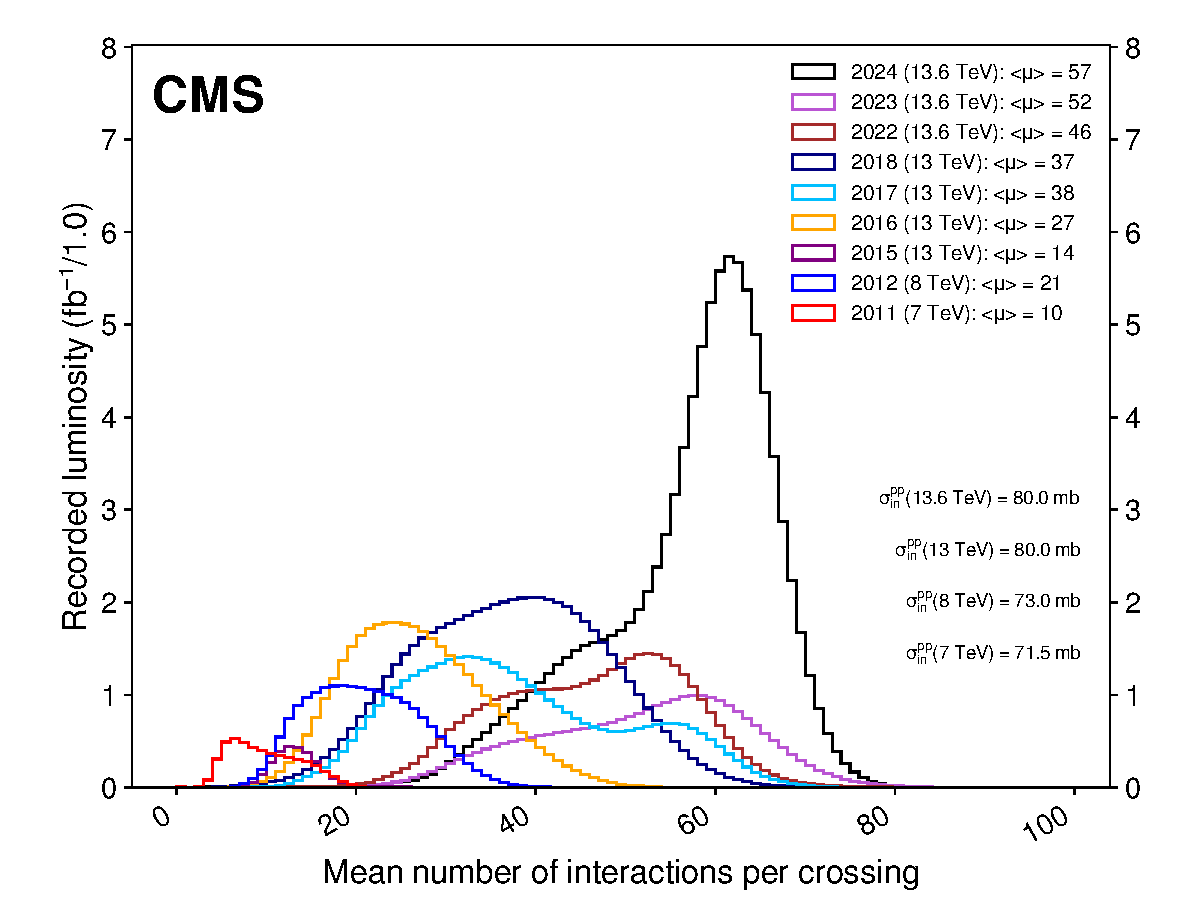
\includegraphics[width=\textwidth]{figures/02-CMS/lhc/pileup_allYears}
    \caption{Mean number of interactions per crossing (pileup) in CMS between 2011--2024, reproduced from Ref.~\cite{cmslumi2024}.}
    \label{fig:02_lhc_pileup}
\end{figure}


\begin{figure}[ht!]
    \centering
    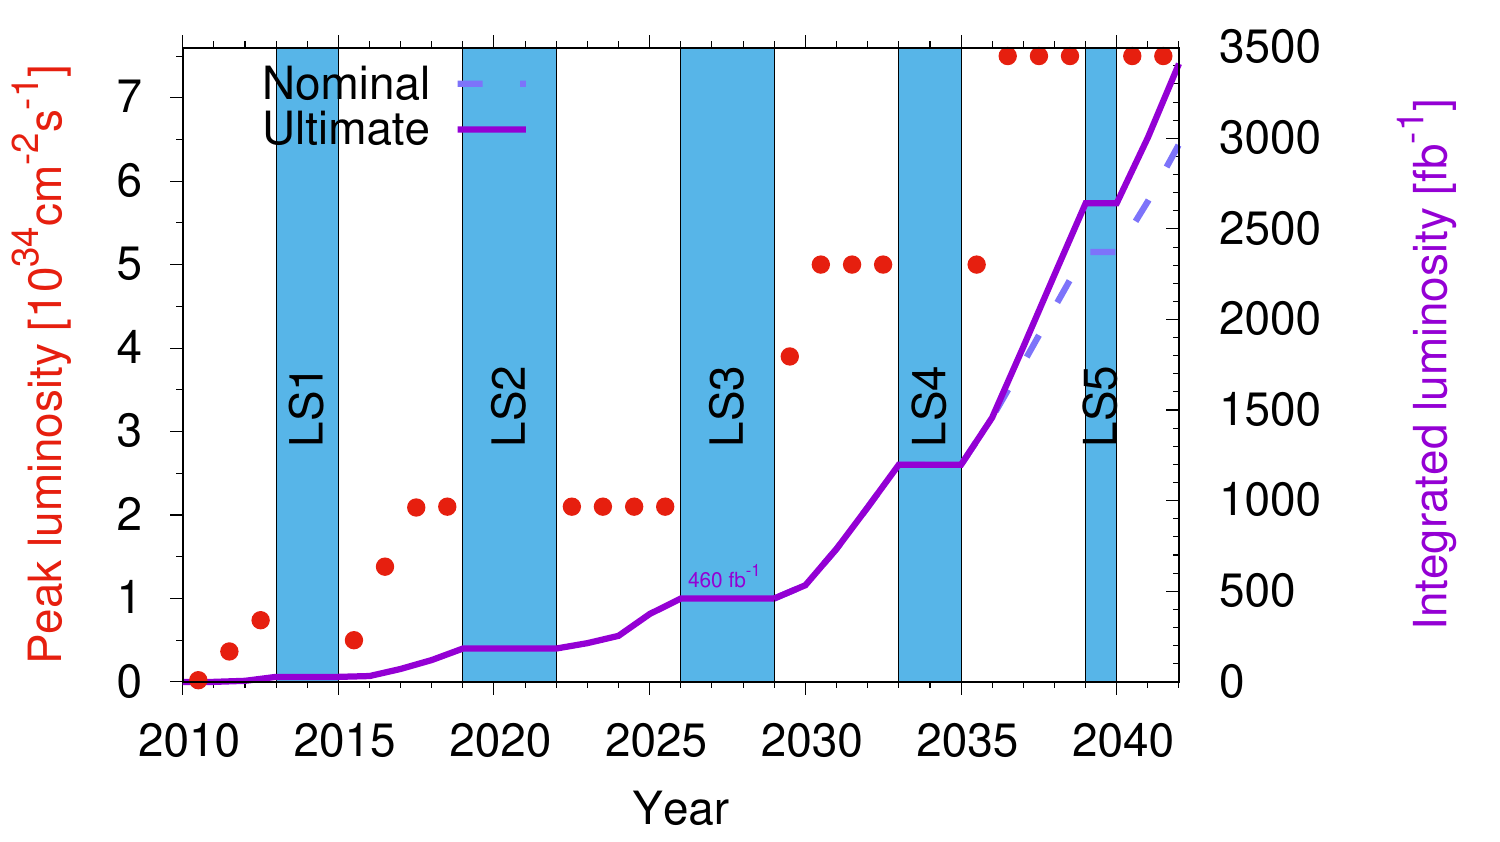
\includegraphics[width=\textwidth]{figures/02-CMS/lhc/luminosity.png}
    \caption{Integrated luminosity delivered by the LHC so far and the projection up to 2041, reproduced from Ref.~\cite{lhclumi}.}
    \label{fig:02_lhc_luminosity}
\end{figure}

\begin{figure}[ht!]
    \centering
    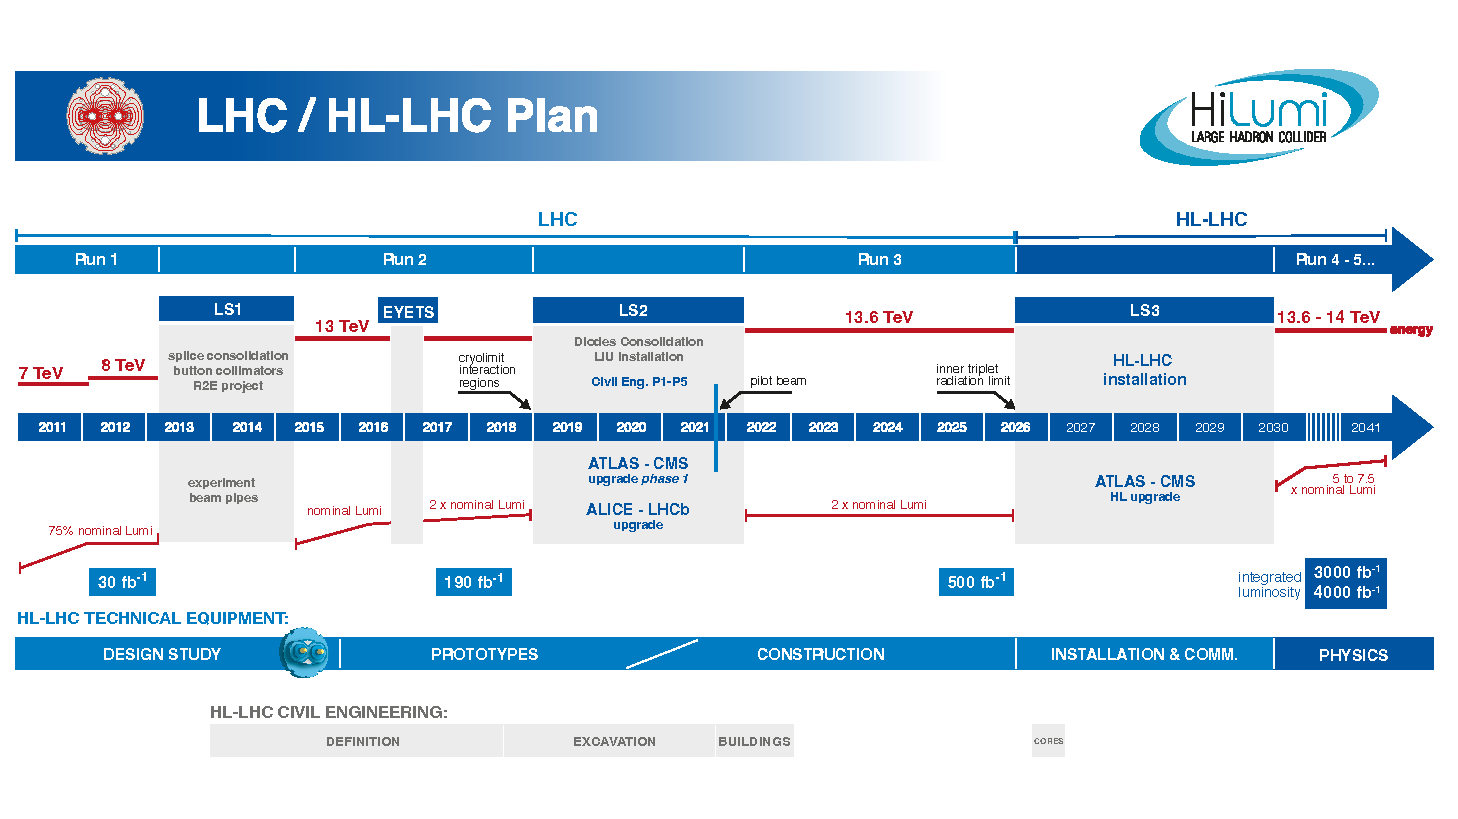
\includegraphics[width=\textwidth]{figures/02-CMS/lhc/HL-LHC_October2024.pdf}
    \caption{The LHC / HL-LHC operation and upgrade plan, reproduced from Ref.~\cite{hllhcplan}.}
    \label{fig:02_lhc_plan}
\end{figure}
